% Beamer Class for presentations
\documentclass{beamer}

% PREAMBLE
\usetheme{Berkeley}
\usecolortheme{seahorse}
\usepackage{graphicx}
\usepackage{subcaption}

% IMAGES FOLDERPATH
\graphicspath{{\_images}{./\_images}}

\title[Computer Science Magazine]{Introducing the Official TUJ Computer Science Magazine}
\subtitle{Welcome to the Magazine Team!}
\author{Bhushith Gujjala Hari}
\institute{Temple University Japan}

\date[Fall 2026]{Fall 2026 Semester, September 2026}

\logo{
\includegraphics[height=1cm]{TUJ_CS_SOCIETY_LOGO.jpg}}

\begin{document}


% ======================
% FORMATTING SECTION START 
% ======================
\AtBeginSection[]
{
    \begin{frame}
        \frametitle{Table of Contents}
        \tableofcontents[currentsection]
    \end{frame}
}



% ======================
% TITLE FRAME
% ======================
\frame{\titlepage}


% ======================
% TABLE OF CONTENTS 
% ======================
\begin{frame}
    \frametitle{Table of Contents}
    \tableofcontents
\end{frame}


% ======================
% SLIDE-1: Intro, what is the TUJ CS Magazine 
% ======================
\section{The TUJ CS Magazine}
\begin{frame}
    \frametitle{TUJ Computer Science Magazine}

    The \textbf{Computer Science (CS) Magazine} will be an offical issue of all of the \textbf{different voices} of the CS community, the students, the developers, the professors, the professionals, and other burning CS topics we want to talk about.

    \hspace{0.4pt}
    \pause

    This is a space where we can express \textbf{ourselves, our creativity, our ideas}, and finally, have an outlet to nerd out about CS topics.  


\end{frame}


% ======================
% SLIDE-1.5: Everyone involved 
% ======================
\section{CS Magazine Team Leaders}
\begin{frame}
    \frametitle{Who leads the Computer Science Magazine Team?}

        \begin{enumerate}

            \item<1-> 
                \textbf{Prof. Hani Karam (CS Supervisor)}: \small{Prof. Karam is a Computer Scientist with research experience in Human Computer Interaction, professional experience as a software engineer.} \pause Prof. Karam will be 

                \begin{itemize}

                    \item<3-> overseeing the entire development of the magazine, 
                    \item<4-> providing advice, 
                    \item<5-> and will be setting the quality threshold for future versions of the magazine. 

                \end{itemize}

            \item<6-> 
                \textbf{Prof. Farid Nakhle (Magazine Supervisor)}: \small{Prof. Nakhle is a Computer Science Professor with more than 15 years of experience in web development, he has also contributed to multiple publications of research in Artificial Intelligence and Biotechnology.} \pause Prof. Nakhle will be 

                \begin{itemize}

                    \item<7-> overseeing the development of the magazine, 
                    \item<8-> reviewing the sections, 
                    \item<9-> handling acknowledgements,
                    \item<10-> and finalizing the post-processing of the magazine before printing. 

                \end{itemize}
 
        \end{enumerate}

\end{frame}

\begin{frame}
    \frametitle{Who leads the Computer Science Magazine Team?}

    \begin{enumerate}

        \item<1-> 
            \textbf{Bhushith Gujjala Hari (Magazine Lead)}: \small{Leader of CS Society. CS and Math Tutor}. 
            \pause I will be 

            \begin{itemize}

                \item<3-> managing deadlines, managing the project, 
                \item<4-> printing, general procedures, 
                \item<5-> and will be leading the magazine team. 
                \item<6-> (Hopefully I'm a good leader! Let me know about any feedback / suggestions). 
                \item<7-> I may also be writing \emph{(depends on how much sleep I can sacrifice)}.

            \end{itemize}

        \item<8-> 
            \textbf{Anastasia Sasaki (Writing Lead \&\& Management)}: \small{Representative of CS Society and experienced writer. She has almost an year of software development experience through her internship and has participated in multiple hackathons}. 
            \pause
            Anastasia will be 

            \begin{itemize}

                \item<9-> overseeing article writing, 
                \item<10-> article sections, article columns, 
                \item<11-> each article's formatting, 
                \item<12-> and general management of the magazine project. 

            \end{itemize}

    \end{enumerate}

\end{frame}



% ======================
% SLIDE-2: What we do? 
% ======================
\section{What we do}
\begin{frame}
    \frametitle{What we do}
        
        \begin{enumerate}
            \item<1-> We give \textbf{voice} to all computer science students to express themselves.
            
            \item<2-> We bring ideas related to Computer Science (CS) from outside the classroom to students within TUJ to inspire them and spark curiosity in them.

            \item<3-> We write meaningful, knowledgeable, and insightful articles that are purely human-made \textbf{(NO A.I., NO LLMs)} to teach everyone about CS.

            \item<4-> We talk to the community, student body, and people in the field to get to know their views, understand their requests, learn from them, and teach the world what we learn. 

            \item<5-> We have some fun along the way!

        \end{enumerate}

\end{frame}


% ======================
% SLIDE-3: What's the plan for this semester?  
% ======================
\section{Plan for this Semester}
\begin{frame}
    \frametitle{What is the plan for this semester?}

        \begin{enumerate}
            \item<1-> We plan what sections should go on the magazine, think of articles we want to write, and vote on the sections.

            \item<2-> We finalize all articles we that want to write.

            \item<3-> We interview people, we talk to field experts, question professors, and reach out to students. 

            \item<4-> We write a few enaging, interesting, and exciting articles, making sure everyone's voice is heard.

            \item<5-> We make them fancy with graphics and design.

            \item<6-> We print them out, share them with everyone (even Non-CS people).
            
            \item<7-> Celebrate!

        \end{enumerate}

\end{frame}


% ======================
% SLIDE-3: Timeline 
% ======================
\section{Magazine Timeline}
\begin{frame}
    \frametitle{Timeline of Making the Magazine}

        Split by Weeks.

        \pause

        \begin{figure}[H]
            \center
            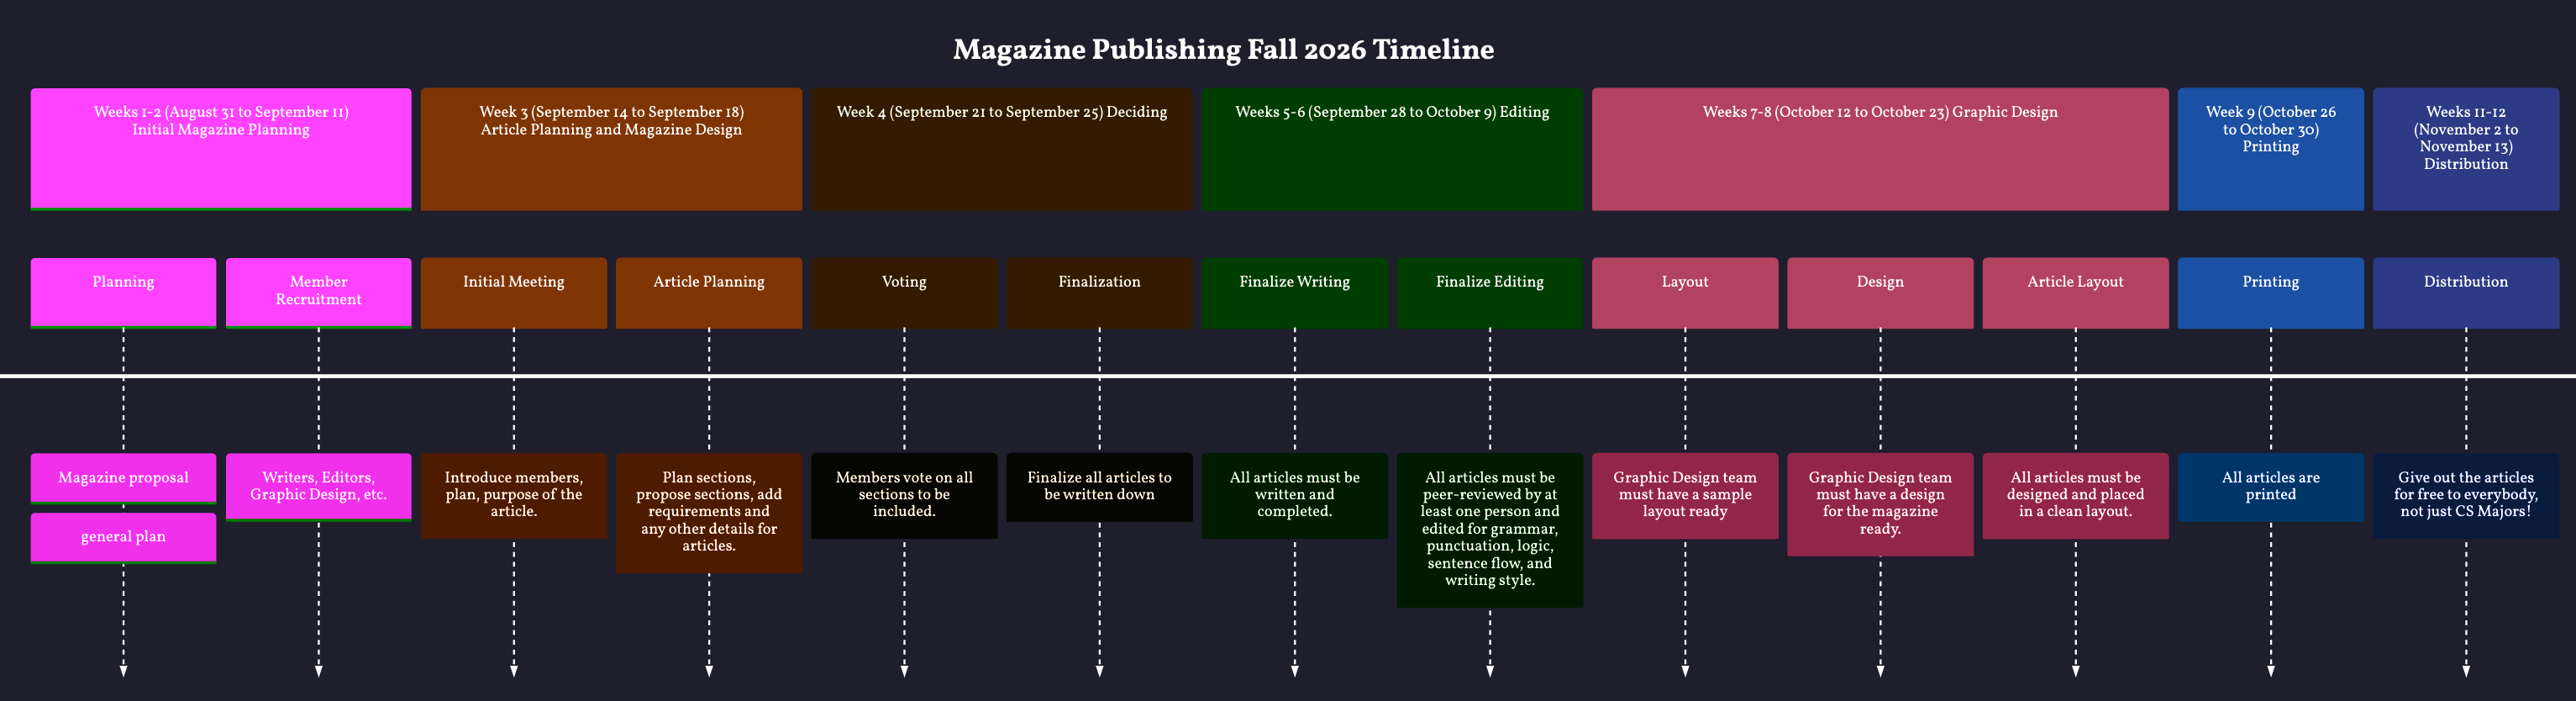
\includegraphics[width=1.0\linewidth]{timeline_full.png}
            \caption{Timeline of the CS Magazine}
            \label{fig:cs-magazine-timeline}
        \end{figure}

\end{frame}

\begin{frame}
    \frametitle{Timeline (cont.) - Kickoff and Planning}
        
        \begin{description}
            \item<1->[Weeks 1-2 (August 31 to September 11)] Initial Magazine Planning
                \begin{itemize}
                    \item<2-> General planning and magazine proposal.
                    \item<3-> \textbf{Member Recruitment}: Writers, Editors, Graphic Design, etc.
                \end{itemize}

            \item<4->[Week 3 (September 14 to September 18)] Article Planning and Magazine Design
                \begin{itemize}
                    \item<5-> \textbf{Initial Meeting}: Introduce members, plan, purpose of the article.
                    \item<6-> \textbf{Article Planning}: Plan sections, propose sections, add requirements and any other details for articles.
                \end{itemize}
        \end{description}
        

\end{frame}

\begin{frame}
    \frametitle{Timeline (cont.) - Writing}

        \begin{description}
            \item<1->[Week 4 (September 21 to September 25)] Deciding and Writing
                \begin{itemize}
                    \item<2-> \textbf{Voting}: Members vote on all sections to be included.
                    \item<3-> \textbf{Finalization}: Finalize all articles to be written down
                    \item<4-> \textbf{Start writing}: Get started on the articles asap!
                \end{itemize}

            \item<5->[Weeks 5-6 (September 28 to October 9)] Writing and Reviewing
                \begin{itemize}
                    \item<6-> \textbf{Finalize Writing}: All articles must be written and completed.
                    \item<7-> \textbf{Review}: Try to get started on article review (at least one peer review by another writer)
                \end{itemize}
        \end{description}   
\end{frame}

\begin{frame}
    \frametitle{Timeline (cont.) - Editing and Design}
        
        \begin{description}
            \item<1->[Weeks 7-8 (October 12 to October 23)]: Editing and Graphic Design
                \begin{itemize}
                    \item<2-> \textbf{Finalize Editing}: All articles must be peer-reviewed by at least one person and edited for grammar, punctuation, logic, sentence flow, and writing style.
                    \item<3-> \textbf{Layout}: Graphic Design team must have a sample layout ready
                    \item<4-> \textbf{Design}: Graphic Design team must have a design for the magazine ready.
                    \item<5-> \textbf{Article Layout}: All articles must be designed and placed in a clean layout.
                \end{itemize}
        \end{description}
\end{frame}

\begin{frame}
    \frametitle{Timeline (cont.) - Printing and Distribution}

        \begin{description}
            \item<1->[Week 9 (October 26 to October 30)]: Printing
                \begin{itemize}
                    \item<2-> \textbf{Printing}: Send out articles for printing. Pray that all articles are printed within 1-2 weeks.
                \end{itemize}


            \item<3->[Weeks 10-12 (November 2 to November 20)]: Distribution 
                \begin{itemize}
                    \item<4-> \textbf{NOTE}: Dates depend on when printing can be completed
                    \item<5-> Give out the articles for free to \textbf{everybody}, not just CS Majors!
                \end{itemize}
        \end{description}

\end{frame}


% ======================
% SLIDE-4: Teams 
% ======================
\section{The Team}
\begin{frame}
    \frametitle{The Team: Who will you be working with?}

        \begin{description}
            \item[Writers]<1-> The writer team consists of people interested in researching and writing articles. You should be ready to interview people, ask around, gather information, research sources, and more to be a writer! 

            \item[Editors]<2-> We don't have a designated editing team because we will be asking each writer to peer review another writer's work! 

            \item[Design]<3-> Design each article's style, layout, format, and give a stylish look and format the magazine.

            \item[General]<4-> The general team will help with everything else that's necessary: Printing, management, budget requesting, fund gathering, keeping up to date with each member, and more!

        \end{description}

        \pause
        \pause
        \pause
        \pause
        \textbf{Each team is EQUALLY important in making this magazine a reality!}

\end{frame}


% ======================
% SLIDE-5: Magazine Sections 
% ======================
\section{Magazine Sections}
\begin{frame}
    \frametitle{Sections of the Magazine}

        Here's what we have planned so far. This is for our budget proposal to the CS department (it doesn't have to be this way).

        \hspace{0.4pt}
        \pause
        
        \begin{itemize}

            \item<2-> \textbf{Tech} Introduce cool, useful, and innovative tech and software to students that might help them in their academic journey or professional career.

            \item<3-> \textbf{Research} Talk about an interesting research paper or article in the CS field, explain its impact, explain why you found it important.

            \item<4-> \textbf{Student Experiences} A section to talk about student experiences, how did you get into CS, what did you do to enjoy your journey in CS, how does staying in Tokyo help that? How did TUJ help you achieve your CS dreams?

        \end{itemize}
\end{frame}

\begin{frame}
    \frametitle{Sections of the Magazine (continued)}

        Here's what we have planned so far. This is for our budget proposal to the CS department (it doesn't have to be this way).

        \hspace{0.4pt}
        \pause
        
        \begin{itemize}

            \item<2-> \textbf{Hackathon and Event Reports} Did you go to a Hackathon or Tech event recently? How was it? What did you do? How did you make the most of it? Talk about your experience, why they're generally fun, and why other people should also give them a try!

            \item<3-> \textbf{Voices}: The voices section features interviews with industry professionals, research experts, active students, experienced tech people, and anyone else you find interesting. Why did you find them interesting? What did you take away from the interview? And, most importantly, what can we learn from this person? 

        \end{itemize}

\end{frame}

\begin{frame}
    \frametitle{Sections of the Magazine (continued)}

        And, finally,

        \hspace{0.4pt}
        \pause
        
        \begin{itemize}

            \item<2-> the articles can be \textbf{ANYTHING you want!} That's \emph{write}! The sections are there to just give you ideas and formalize the magazine a bit, there's no need to follow exactly any of the articles mentioned previously

        \end{itemize}

\end{frame}




% ======================
% SECTION: THANK YOU 
% ======================
\begin{frame}
    \frametitle{Thank you for your time!}

    Thank you for listening to this presentation! 
    \pause

    Thank you for joining us and being part of this dream of ours!
    \pause

    Thank you for your time, interest, commitment, and dedication!
    \pause


    and with that,
    \pause

    \hspace{0.4pt}


    Welcome to the Computer Science Magazine Team! 
\end{frame}

\begin{frame}
    
    \frametitle{Next Agenda}

    \begin{enumerate}
        
        \item<1-> Think of a Magazine Title: OwlBytes, OwlCommit, etc. (you can thank me for the horrible name ideas).

        \item<2-> Think of what YOU wanna write!

        \item<3-> Get started on writing, we have very little time.

    \end{enumerate}

\end{frame}








\end{document}

